\section{Conclusion}

To address the change of its scope from electron to pion identification for momenta
greater than 3.5 GeV, the LTCC has been refurbished. The work included improvements of the
reflectivities for the mirrors and the Winston cones, p-terphenyl
coating of the PMTs, expansion of the gas volumes, and redesign of the box walls and patch panels.
The LTCC detector sectors after refurbishment are show in \F{ltccInstalled}.
Performance conclusion here too.

\begin{figure}
	\centering
	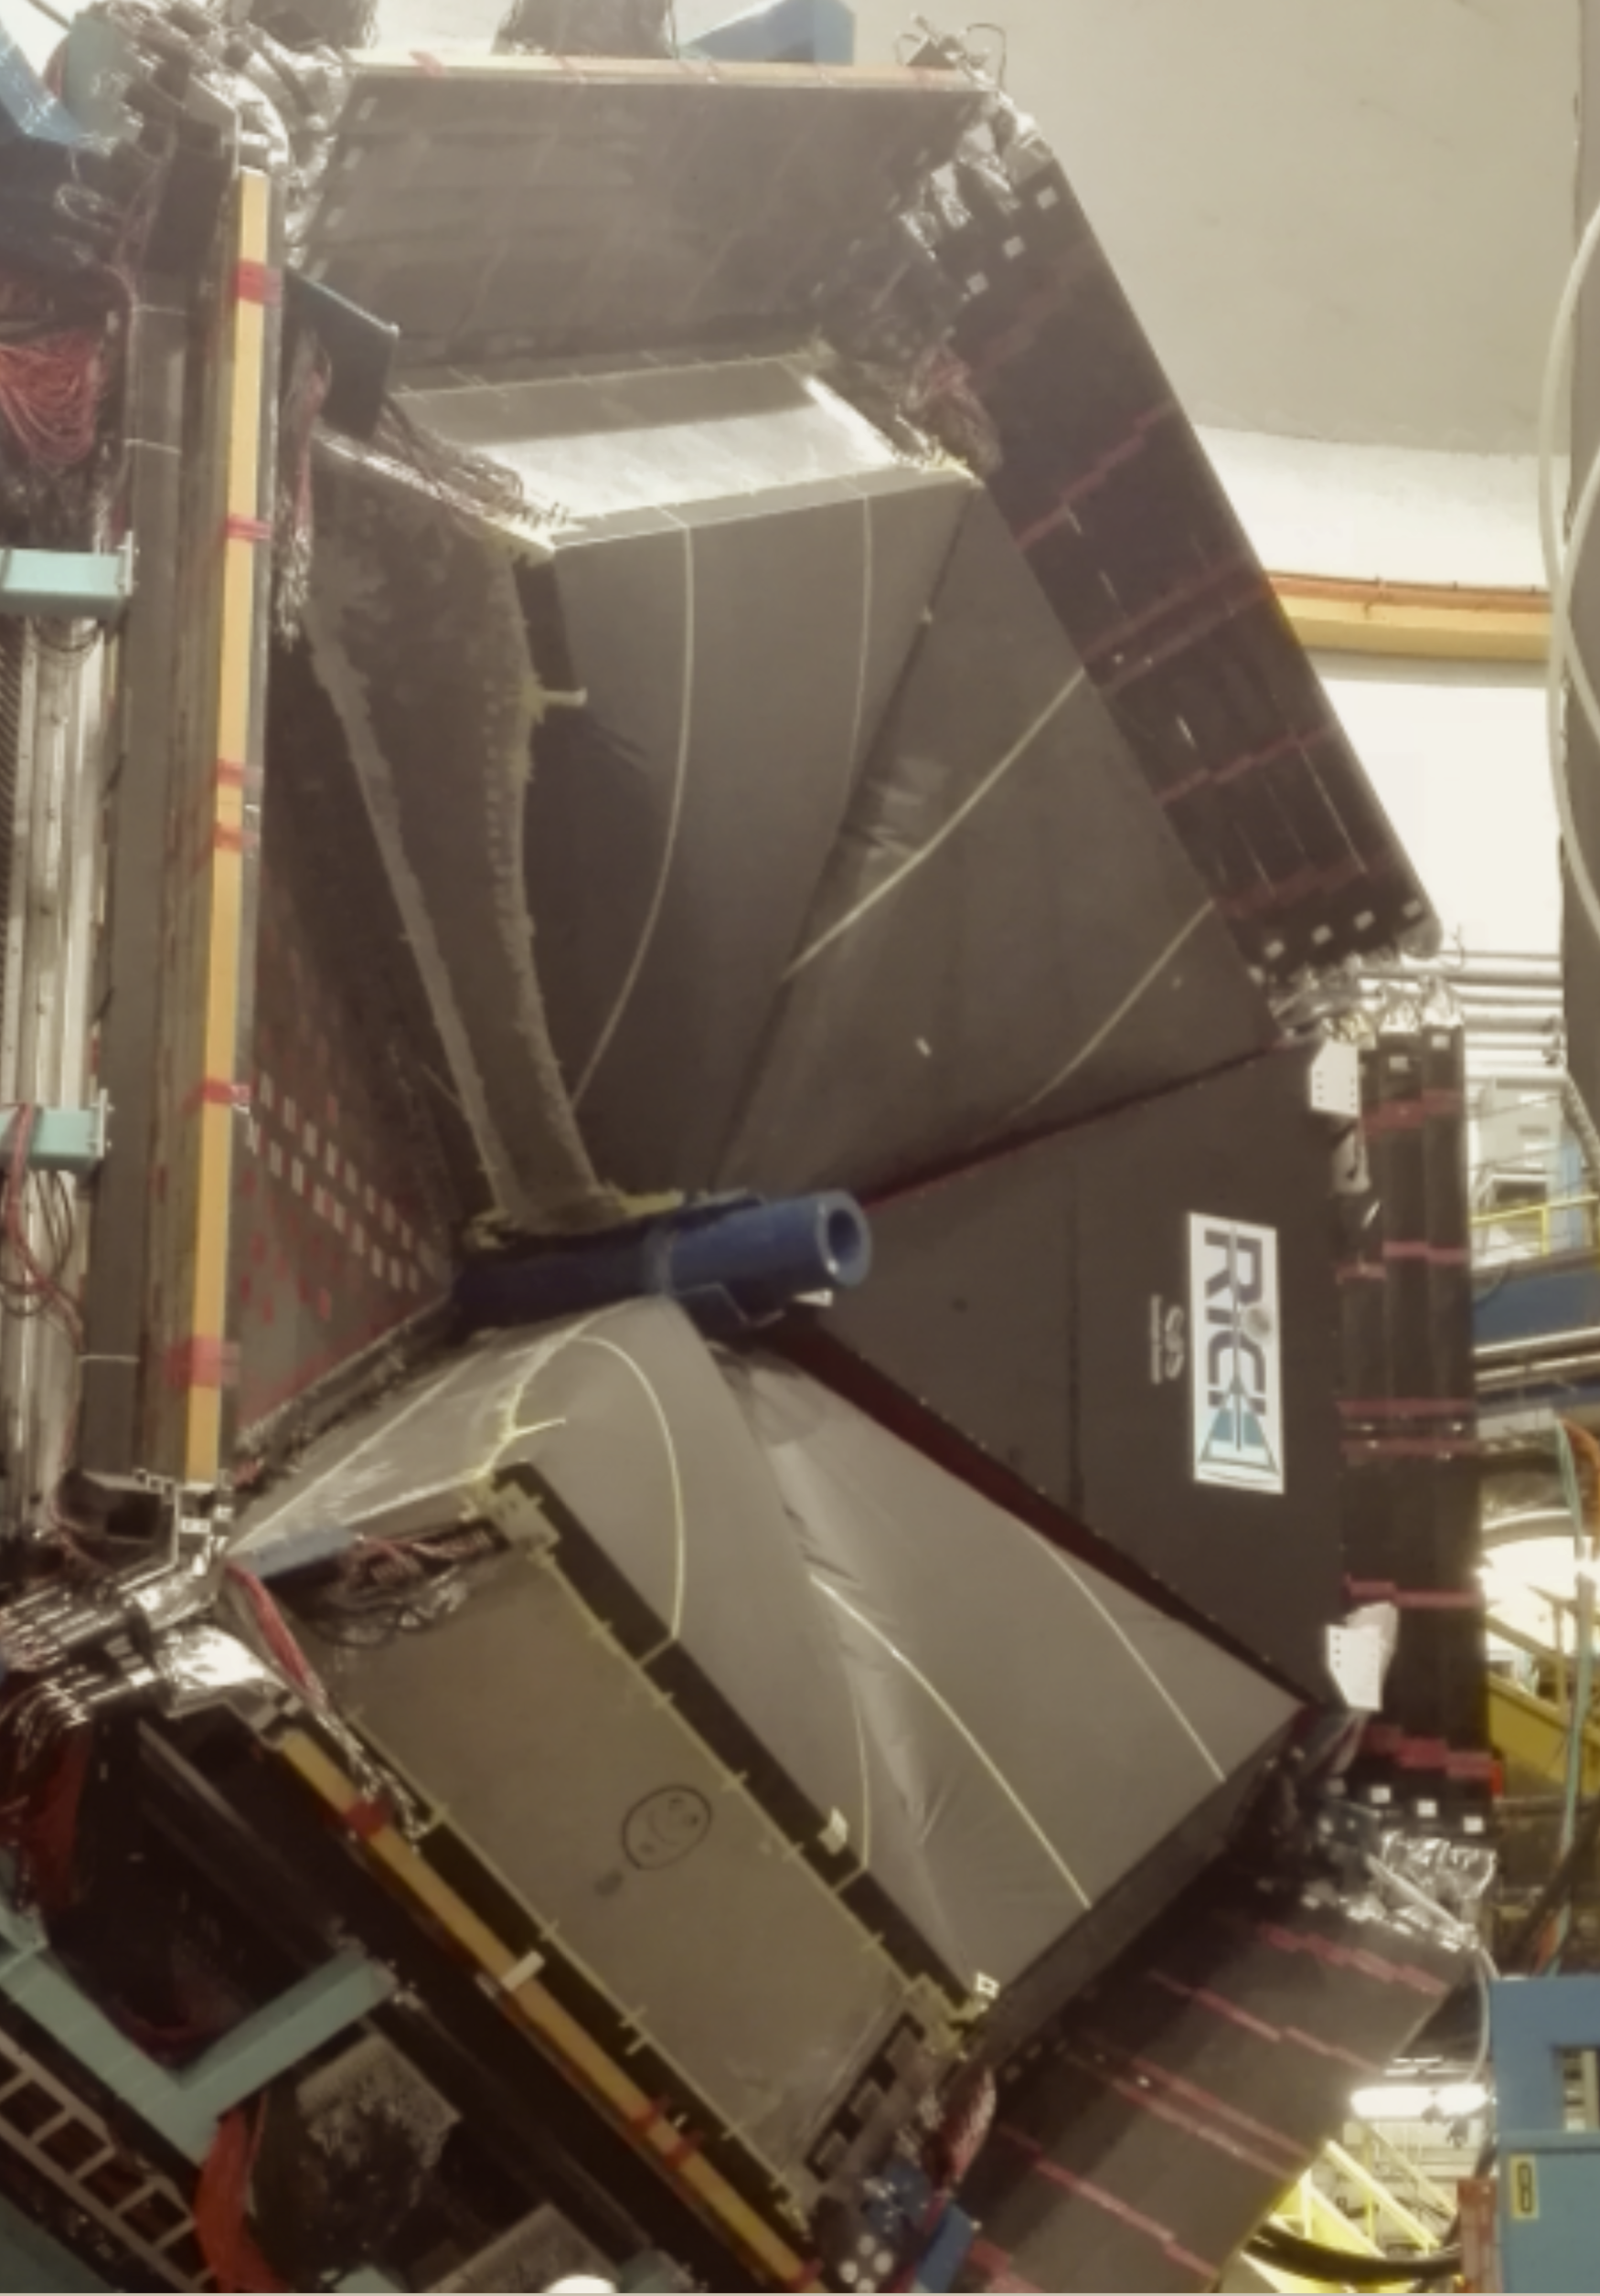
\includegraphics[width=1.0\columnwidth,keepaspectratio]{img/ltccInstalled.png}
	\caption{The LTCC sectors installed after refurbishment on the CLAS12 Forward Carriage.}
	\label{fig:ltccInstalled}
\end{figure}


\section{Acknowledgments}

We thank the Detector Support Group at Jefferson Lab for the work on the cone refurbishment, reflectivity tests,
PMT divider modifications and installation, and for designing the gas control system and associated software.
We thank Temple University for the p-terphenyl deposition. We thank Vladimir Popov for the implementation
of the divider base modification. We thank Youri Sharabian and Steve Christo for their consultations and contributions.
We thank the Tech team of Hall B for their work and dedication on all aspect of the project.
Finally, we thank all the Hall B staff for their unyielding support.
This work was supported in part by DOE Contract DE-AC05-84ER40150.

